\subsection{Introduction to Machine Learning}
\label{subsect: intro to ML}
Machine learning is a field of artificial intelligence that enables computers to learn patterns and make decisions based on data without being explicitly programmed to do so. Where artificial intelligence is field of research in computer science which aims to develop machine intelligence, such as the ability to interact with the environment, collect and interpret data, learn from this data and make context adapted decisions \cite{danie2021}. Meaning that machine learning is a subset of the concept of artificial intelligence.

Machine learning models can essentially be expressed as a function $\boldsymbol{y}(\boldsymbol{x})$ which takes an input vector $\boldsymbol{x}$ and transforms it to an output vector $\boldsymbol{y}$. The precise form of $\boldsymbol{y}(\boldsymbol{x})$ is determined during the \textit{training phase} on the basis of the training data \cite{bishop2007}. The specific goal of machine learning is to use knowledge drawn from data to make predictions on new unseen data. During the training phase the aforementioned function $\boldsymbol{y}(\boldsymbol{x})$ is formed, the form of this function will depend on: the type of machine learning algorithm, the hyperparameters of the algorithm and the data the function was trained on. Hyperparameters are parameters that can not be changed by the learning algorithm and have to set before the training takes place. Examples of hyperparameters are: batch size, learning rate or topology and size of a neural network.

\begin{figure}[h]
    \centering
    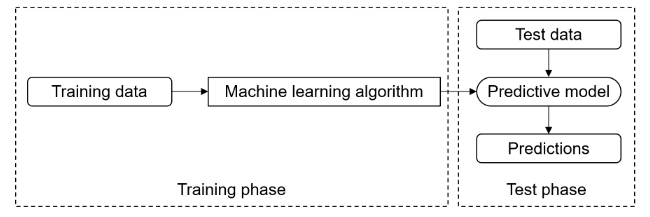
\includegraphics[width=0.75\linewidth]{figures//Literature review/ML_pipeline.png}
    \caption{Training and test phases of a general machine learning model, adapted from \cite{danie2021}}
    \label{fig: MLtraing}
\end{figure}


\subsubsection{The Dataset}
In machine learning, data is typically represented as a large collection of labelled examples \\
$\{(\boldsymbol{x}_1, y_1), (\boldsymbol{x}_2, y_2), \ldots, (\boldsymbol{x}_N, y_N)\}$ where each element $\boldsymbol{x}_i$ is called a feature vector and  $\boldsymbol{y}_i$ is its corresponding label. A feature vector is a vector where each dimension $j$ from 1 to D contains a value that describes the example. Each such value is called a feature and is typically denoted as $x^(j)$. For example if we have a dataset comprised of cars, features could be the length, engine power or colour of the car. For every feature vector $\boldsymbol{x}_i$, the feature at position $j$ will describe the same information \cite{burkov2020}. 

The labels $y_i$ are used to train the machine learning model, they can be an element belonging to a finite set, a real number or more complex structures like vectors or matrix. In the case of the example we just used the labels could be something along the lines of: van, truck, sedan or sports car. 

The machine learning model is trained using data from which features have been extracted and have been labelled beforehand to provide a ground truth on which the model can asses itself. The dataset is typically split into three distinct sets: the training set, validation set and test set. The training set is usually the largest portion and is used to fit the model, allowing it to learn the underlying patterns of the data and to construct the function $\boldsymbol{y}(\boldsymbol{x})$. The validation set is important during training to help fine-tune the hyperparameters of the model after it has been trained on the training set. The validation set provides an unbiased evaluation of the model's performance and can not be seen by the model in the training phase.

\begin{figure}[h]
    \centering
    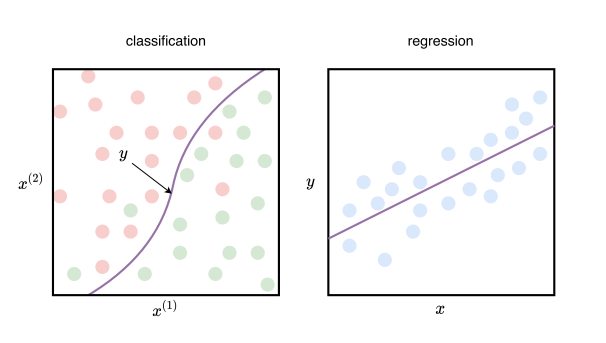
\includegraphics[width=0.75\linewidth]{figures//Literature review/classification_regression.png}
    \caption{Difference between classifier and regressor models, adapted from \cite{burkov2020}}
    \label{fig: classifier-regressor}
\end{figure}

In machine learning, a distinction is made between 2 different models. These being regression and classification models. These models are used for different types of prediction tasks each. A regression models is used when the target we are trying to predict is a continuos value, such as the weight or height of a person. The goal of a regression model is to find a function $\boldsymbol{y}(\boldsymbol{x})$ that can estimate numerical outputs based on the input features. On the other hand, classification models are used when the target consists of discrete categories or classes. Such as determining the type of a car in an image, or if an email is spam or not. The approach to training, evaluating and selecting models can differ between these two, since the type of output and error metrics are not entirely the same. For more information on the model selection and which type of ML model is best suited for which task, please see the works of \textcite{bishop2007, burkov2020}. The difference between these two types of models is seen in \autoref{fig: classifier-regressor}

\begin{figure}[h]
    \centering
    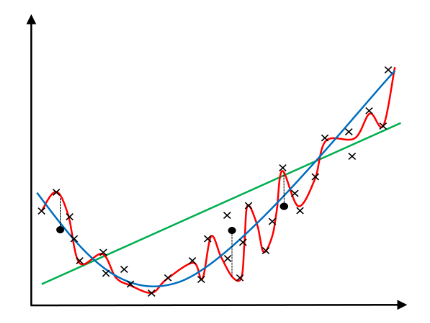
\includegraphics[width=.5\linewidth]{figures//Literature review/overfitting.png}
    \caption{Graphical representation of overfitting (red line) and under fitting (green line) for a regression problem. Training data is represented with crosses and test data are dots. Adapted from \cite{danie2021}}
    \label{fig: overfitting}
\end{figure}

Machine learning models can sometimes exhibit a problem called overfitting, where the ML model has been trained to have a very high accuracy on the training data, which will lead to bad predictions on unseen test data. Overfitting can be caused by badly configure hyperparameters or or too few training examples. The opposite of overfitting can also occur, which is when the model is not correctly following the training data and exhibits a fit that is too general. Examples of these problems can be seen in \autoref{fig: overfitting}

\subsubsection{Types of Machine Learning}
In general machine learning can be classified into 3 different categories, namely \textbf{supervised}, \textbf{unsupervised} and \textbf{reinforcement} learning \cite{bishop2007, burkov2020, danie2021}.

\begin{itemize}
    \item \textbf{Supervised Learning}: every database entry $\boldsymbol{x}$ is associated to a label $y$ and the model will learn the correspondence between them. The output can be either categorical (classification), or numerical with a continuous set of possibilities (regression) \cite{danie2021}.
    \item \textbf{Unsupervised Learing}: the training data is not labelled at all. The goal of this model type is to uncover hidden patterns, structures or relationships in the data. Examples are K-mean clustering or principal component analysis (PCA) which is closely related to POD. 
    \item \textbf{Reinforcement Learning} is where an the algorithm learns to make decisions by interacting with an environment. Here an agent will interact will recieve rewards or penalties based on its actions and aims to learn a sequence of decisions that will maximize a cumulative reward. Examples are self driving cars or software that can play games like AlphaGO \cite{alphago2023}.
\end{itemize}


\subsection{Introduction to Neural Networks}
Neural networks (NNs) are a class of machine learning techniques inspired by the biological nervous system, simulating how learning occurs in a living organism. They consist of interconnected computational units, or neurons, which receive inputs, process them through an activation function and produce an output. A general architecture of a NN can be seen in \autoref{fig: FNN}, where the NN displays an input layer on the left, hidden layers in the middle and an output layer on the right. A network where information flow follows this path is called a feed forward neural network or FNN \cite{Aggarwal2018}.

\begin{figure}[h]
    \centering
    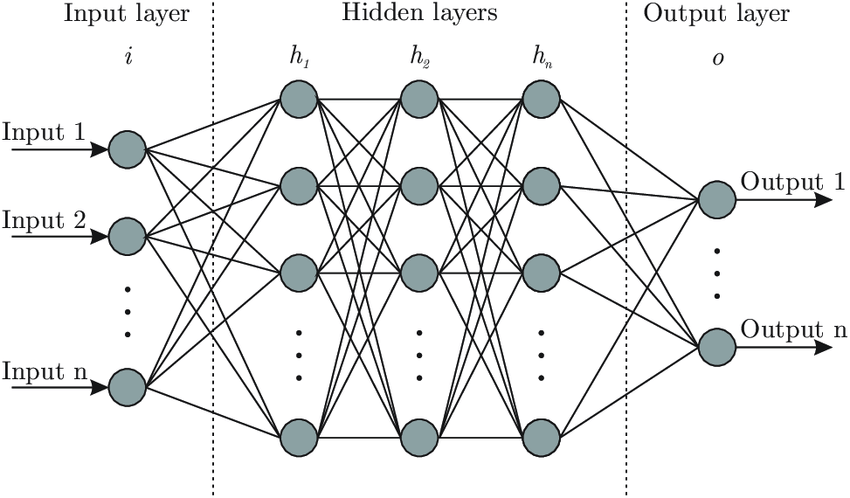
\includegraphics[width=0.8\linewidth]{figures/Literature review/NeuralNetwork.png}
    \caption{General architecture of a Feed Forward Neural network, adapted from \cite{nashtech_activation2023}}
    \label{fig: FNN}
\end{figure}
Neural networks are one of the most used machine learning paradigms because of their advanced capabilities and performance in handling complex fluid phenomena \cite{Brunton2020}. That is why this subsection aims to build on the machine learning basics which have been laid in \autoref{subsect: intro to ML} and serve as an additional basis to how neural networks have been implemented in CFD workflows. 

\subsubsection{Working Mechanism of Neural Networks}
Mathematically, a single neuron performs a weighted sum of the inputs it receives from the preceding layer. For an input vector $\mathbf{x} = [x_1, x_2, \dots, x_n]$, where the size of the input vector depends on the size of the input layer, the output $\hat{y}$ of a single neuron is computed using \autoref{eq: neuron}

\begin{equation}\label{eq: neuron}
    \hat{y} = \phi\left(\sum_{i=1}^{n} w_i x_i + b\right)
\end{equation}

Where $w_i$ are the weights, $b$ is the bias term and $\phi()$ is the activation function. The activation function determines how the neuron should be activated or not, by choosing the right activation function non-linearity can be introduced into the network outputs. Without this activation function the neural network would just behave like a linear model. Common activation functions include the ReLU (Rectified Linear Unit), sigmoid and tanh \cite{Aggarwal2018}. Where ReLU is particularly popular in deep neural networks due to its simplicity and performance benefits. This type of weighted sum is then executed for every node in the network to eventually produce a prediction at the output layer. 

It is because of this ability to exhibit non linear capabilities that neural networks can be seen as universal function approximators. This concept was established by \textcite{Hornik1989} where the Universal Approximation Theorem was first proposed. In this work the author sates that: "a standard multilayer feedforward network, such as depicted in \autoref{fig: FNN}, with as few as one hidden layer can approximate any Borel to any desired degree of accuracy, proved sufficiently many hidden units are available" \cite{Hornik1989}. The key to this power lies in the use of non linear activation functions, like the ones which have just been discussed. While a single hidden layer might be sufficient in theory, in practice deeper models are preferred as they reduce the number of required network parameters to achieve a desirable solution\cite{Aggarwal2018}. This powerful capability is why neural networks are frequently implemented in tasks where there is a wish to approximate intricate functions, such as in CFD. This strong capability will be highlighted more in later sections in this work. 

If we consider a node on the output layer of the network, the right side of \autoref{fig: FNN}, the output of the neurons $\hat{y}_n$ is the actual prediction of the neural network. If the correct output of the value were to be $y$, the error of the prediction is therefore $E(\mathbf{x})= y-\hat{y}$. In cases where the error value is non-zero, the weights of the neural network need to be updated in such a way that the error can be minimized \cite{Aggarwal2018}. 

The loss function $J(\theta)$ represents the average discrepancy between the predicted output and the true output over all training examples, it follows the general formulation as seen in \ref{eq: loss}.

\begin{equation}\label{eq: loss}
    J(\theta) = \frac{1}{m} \sum_{i=1}^{m} \mathcal{L}(\hat{y}^{(i)}, y^{(i)})
\end{equation}

\begin{wrapfigure}{r}{0.5\textwidth}
    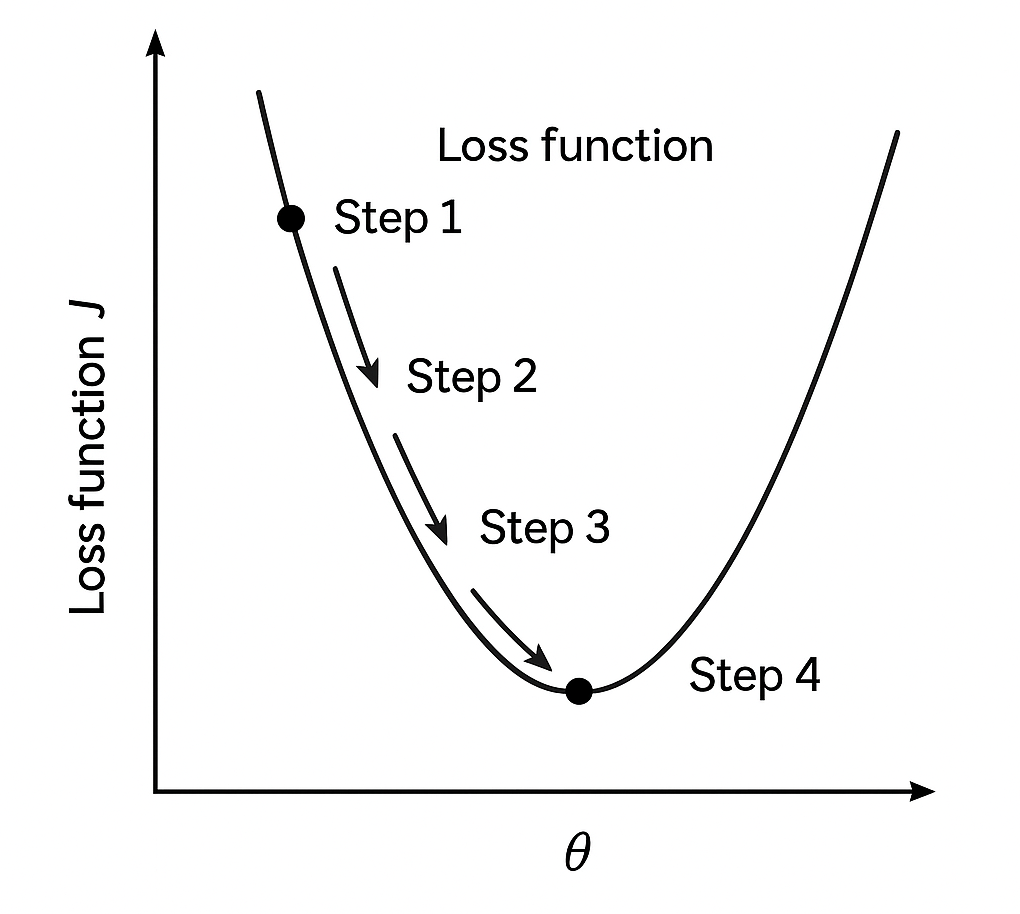
\includegraphics[width=0.8\linewidth]{figures/Literature review/gradient_descent.png}
    \caption{General overview of gradient descent}
    \label{fig: gradientdescent}
\end{wrapfigure}

Where $\theta$ resembles the set of all trainable parameters (such as weights and biases) $m$ is the number of training samples in the database and $\mathcal{L}(\hat{y}^{(i)}, y^{(i)})$ is the individual loss incurred on the $i$-th training sample. By changing the weights and biases of every node the loss function can be minimized, which equates to a more accurate machine learning model. The function $\mathcal{L}$ is chosen depending on the nature of the learning task, mean squared error (MSE) is a famous example. 

The minimisation of the loss function is most frequently achieved through a gradient descent algorithm and its variants \cite{Aggarwal2018}. This is an iterative optimisation process where the parameters of the network are updated such that the error of the model moves in the opposite direction of the gradient of the loss function \cite{Aggarwal2018}, a graphical representation of this can be seen in \autoref{fig: gradientdescent}. The determination of the gradient of the loss function is achieved through a process known as backpropagation. This algorithm applies the chain rule of over the nodes of the network to efficiently compute the gradient of the loss function with respect to each trainable parameter in the network (which is represented by $\theta$). Backpropagation starts from the output layer and and propagates the error backwards through the network, where it calculates the local gradient at each layer by multiplying the derivative of the the activation function with the error signal. If this process is repeated for every path through the network to determine the eventual gradient of the loss function $\frac{\partial J}{\partial \theta}$. This gradient can then be used to update the network parameters using the \autoref{eq: gradient descent}


\begin{equation}\label{eq: gradient descent}
    \theta := \theta -\alpha \frac{\partial J}{\partial \theta}
\end{equation}

Where $\alpha$ is the learning rate, it essentially determines the speed at which the loss function is minimized with and plays a key role in the time it takes to train the model. 

\subsection{Common Neural Network Architectures Employed in CFD}
\label{subsect: commonNN}
Before an overview can be made on how neural networks have been implemented in CFD workflows, it is useful to first outline the most frequently used neural network architectures in the CFD landscape. This part of the literature review will briefly introduce the foundational neural network architectures most commonly applied in CFD applications, which will serve as a foundation for understanding their role in data-driven fluid dynamics. 

\subsubsection{Feed-Forward Neural Networks}
Feed-Forward neural networks (FNNs) are essentially the most basic form of neural networks, their general architecture is displayed in \autoref{fig: FNN}. As mentioned beforehand, information flows in one direction from input to output. They can be simple and contain just a few hidden layers, which is sometimes referred to as a shallow network. FNNs can also contain higher number of hidden layers, which is referred to as a deep neural network \cite{Aggarwal2018}. 

One interesting use of FNNs in scientific computing are Physics Informed Neural Networks (PINNs). First proposed by \textcite{Raissi2019}, PINNs aim to integrate neural networks with fundamental physical laws to solve differential equations. The original work explains the concept by approximating a function $u(t, x)$ with a neural network, where the loss function is constructed from 2 main components: a term derived from data, and a physics informed term. that enforces the governing differential equations and relevant boundary conditions. This way PINNs can enforce consistency to information it has learned from data, and to governing physical laws. By utilizing the ability of neural networks to act as universal function approximators \cite{Hornik1989}, PINNs can represent complex physical fields and solution manifolds with high accuracy. In the original work PINNs have been used to approximate various famous PDE's, such as the NSE, Schr\"odinger equation and the Allen-Cahn equation with errors close to machine precision \cite{Raissi2019}. 

\subsubsection{Convolutional Neural Networks}
Convolutional Neural Networks (CNNs) are a frequently used class of neural networks specifically designed to process grid-structured input data that exhibit strong spatial dependencies in local regions of the grid \cite{Aggarwal2019}. That is why CNNs are often used for image recognition, since adjacent spatial locations in an image often have similar color values of the individual pixels. CNNs are characterised by convolution operations, which involve taking a dot-product between grid-structured set of weights (known as a filter or kernel) which are used to extract features from the input data. 


\begin{figure}[h]
    \centering
    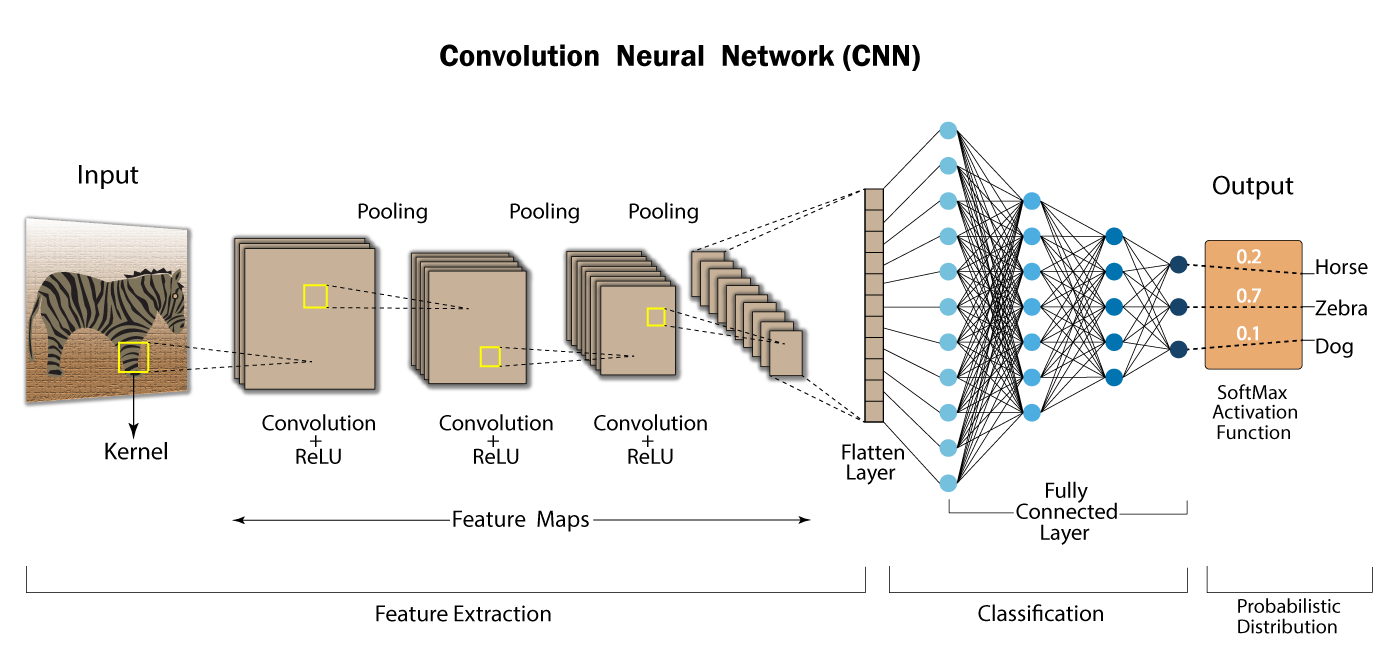
\includegraphics[width=\linewidth]{figures//Literature review/cnn2.png}
    \caption{Overview of the architecture of a convolutional neural network, adapted from \cite{developersbreach}}
    \label{fig: CNN}
\end{figure}

CNNs function much like traditional FNNs, except that the operations in its layers are spatially organized with carefully designed connections between layers. The three types of layers that are commonly present in CNNs are convolution, pooling and ReLU, which can be seen in \autoref{fig: CNN}. These layers are used to extract features from the and reduce the number of trainable parameters in the network. By applying these filters spatially invariant patterns can be extracted such as edges, corners or textures. This all happens in the feature extraction part of the network, before the filtered data is used as input for the classification part of the network, shown on the left and right of \autoref{fig: CNN} respectively. 

CNNs have shown outstanding results for image processing tasks, mainly due to their architecture being specifically designed for the relevant domain they want to classify. Because of this strong performance, several well-established CNN architectures have been developed and made publicly available, allowing them to be adapted for specific use cases. Architectures such us AlexNet, LeNET-5 and GoogLeNet are notable examples of predetermined architectures that have shown great results across a various cases of computer vision applications \cite{Alzubaidi2021}.

Because of the strong capabilities of CNNs to extract features out of image snapshots, they present themselves as good candidates to be implemented for CFD predictions. Since CFD flow fields can be represented as structured grid, CNNs offer a great possibility to effectively learn patterns such as vortices or boundary layers. This can prove useful for tasks like flow prediction, surrogate modelling or acceleration \cite{Lee_You_2019, Guo2016}.